In the previous section, we demonstrated that we can train a model to in-context learn linear functions with respect to the distribution of prompts encountered during training.
That is,  we evaluate the in-context learning ability of the model with respect to distributions $D_\mathcal{X}$ and $D_\mathcal{F}$ that were also used to train the model.

Here, we evaluate the in-context learning performance of our model on prompt distributions different from the one used for training.
Our overarching goal here is to better understand the learning algorithm encoded by our model by analysing how it responds to different prompt distributions.

Formally, we will refer to the distribution of functions used during training as $D_\mathcal{F}^\text{train}$ and the corresponding distribution of prompt inputs as $D_\mathcal{X}^\text{train}$.
Then, during inference, functions are sampled from a (potentially different) distribution $D_\mathcal{F}^\text{test}$, while prompt inputs from a distribution $D_\mathcal{X}^\text{test}$.
Moreover, deviating again from our analysis so far, we also consider a separate distribution  $D_\text{query}^\text{test}$, from which the query input is sampled, potentially dependent on the rest of the in-context inputs $x_1,\ldots,x_k$ (which are still sampled from   $D_\mathcal{X}^\text{test}$).

Within this framework, we consider the same model as last section, and evaluate its performance on prompts that deviate from those encountered during training, either by
\begin{enumerate}
    \item sampling prompt inputs or functions from a different distribution, that is $D_{\mathcal{X/F}}^\text{train}\neq D_{\mathcal{X/F}}^\text{test}$ or
    \item introducing a mismatch between in-context examples and the query input, that is $D_\text{query}^\text{test} \neq D_\mathcal{X}^\text{test}$.
\end{enumerate}
We describe each such prompt structure below and present a subset of the results in Figure~\ref{fig:distribution} (see Appendix~\ref{app:dist_shift} for additional details and full results). 
Overall, the model performs reasonably accurate in-context learning with respect to these prompt distributions, indicating that it has indeed learnt to perform linear regression to some generality.

Recall that we generate a training prompt $P = (x_1, w^T x_1,   \ldots, x_k, w^T x_k, x_{\text{query}})$ by drawing the prompt inputs ($x_i$ and $x_{\text{query}}$), and the weight vector ($w$) i.i.d.\ from $N(0, I_d)$, with $d = 20$. For all the settings below, except prompt scaling, we normalize the inputs so that their expected squared norm is equal to that of inputs encountered during training. 

\begin{figure}[htp]
    \centering
    \begin{subfigure}[b]{0.33\textwidth}
        \centering
        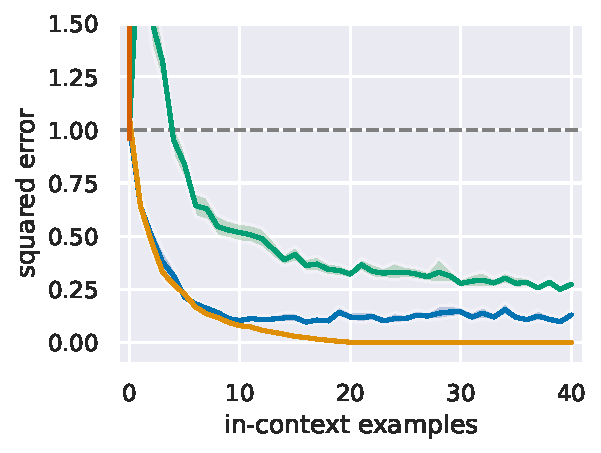
\includegraphics[height=.75\textwidth]{figures/skewed.pdf}
        \caption{Skewed covariance}
        \label{fig:skewed}
    \end{subfigure}
    \begin{subfigure}[b]{0.33\textwidth}
        \centering
        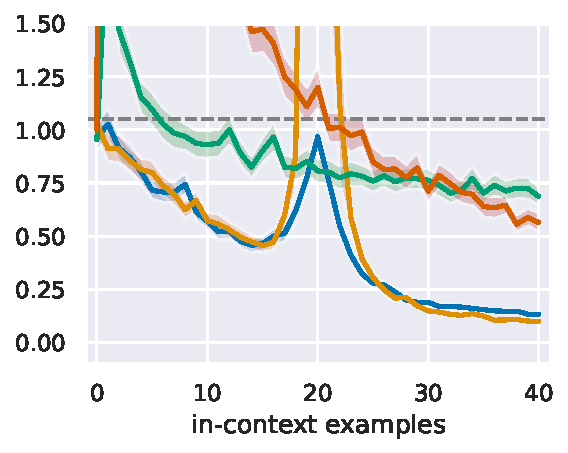
\includegraphics[height=.75\textwidth]{figures/noisyLR.pdf}
        \caption{Noisy linear regression}
        \label{fig:noisy}
    \end{subfigure}
    \begin{subfigure}[b]{0.33\textwidth}
        \centering
        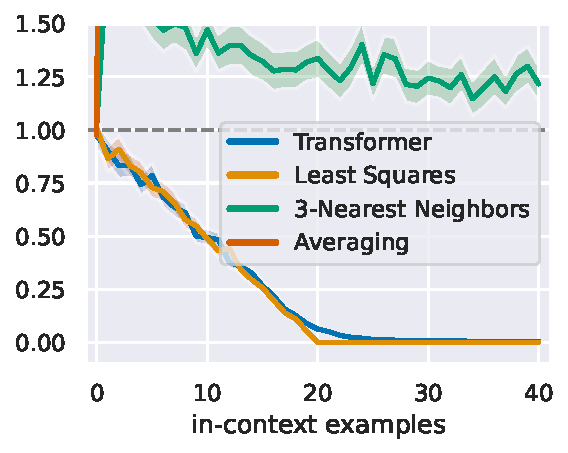
\includegraphics[height=.75\textwidth]{figures/random.pdf}
        \caption{Different orthants}
        \label{fig:random}
    \end{subfigure}
    \caption{\emph{In-context learning on out-of-distribution prompts.}
    We evaluate the trained model on prompts that deviate from those seen during training by: 
    (a) sampling prompt inputs from a non-isotropic Gaussian,
    (b) adding label noise to in-context examples,
    (c) restricting in-context examples to a single (random) orthant.
    In all cases, the model error degrades gracefully and remains close to that of the least squares estimator, indicating that its in-context learning ability extrapolates beyond the training distribution.
    }
    \label{fig:distribution}
\end{figure}

\paragraph{Skewed covariance.} We sample prompt inputs from $N(0, \Sigma)$ where $\Sigma$ is a skewed covariance matrix with eigenbasis chosen uniformly at random and $i^{\text{th}}$ eigenvalue proportional to $\nicefrac{1}{i^2}$.
The model matches the performance of least squares until $k=10$, mimicking the sharp drop in the error in this regime, but its error plateaus afterwards (see Figure \ref{fig:skewed}). 
Thus, it is not perfectly robust to this distribution mismatch but still does relatively well, achieving less than half the error of the nearest neighbor baseline in most cases.

\paragraph{Low-dimensional subspace.} We sample prompt inputs from a random $10$ dimensional subspace. 
In this case, the model achieves low error after 10 in-context examples,  closely matching the behavior of the optimal least squares estimator (the model achieves an error of $0.036$, $0.0014$, and $0.00057$ at 10, 20, and 40 in-context examples respectively)---see Appendix Figure \ref{fig:half_app}.
Crucially, unlike the training prompts, when $k$ is between $10$ and $20$, the prompt inputs are linearly dependent, and a model  achieving low error in this regime indicates that it encodes a valid orthogonalization procedure for these inputs.
% 10 20 40
%half [0.03663731813430786, 0.0013808086514472961, 0.0003733177436515689]
%std [0.5128405094146729, 0.020673632621765137, 0.0005758586339652538]

\paragraph{Noisy linear regression.} We add noise to each prompt output, that is, the $i^{\text{th}}$ output is equal to $w^T x_i + \epsilon_i$ where $\epsilon_i \sim N(0, 1)$.
The trained model closely tracks the performance of least squares when the number of in-context examples is not close to the input dimension $20$ (see Figure \ref{fig:noisy}). 
Interestingly, the model also exhibits the double descent error curve~\citep{belkin2019reconciling}  that is known to manifest for the least squares estimator~\citep{nakkiran2019more}.
Note that in this noisy setting, the optimal estimator corresponds to solving least squares with appropriate $\ell_2$-regularization. However, since the model was trained on noiseless data, we cannot expect it to learn this.

\paragraph{Prompt scale.} We consider the setting where the prompt scale between training and inference is different. We either scale the prompt inputs or the weight vectors, by a factor $\{\nicefrac{1}{3}, \nicefrac{1}{2},  2, 3\}$.
The model is relatively robust when scaling the weight vector, but not as robust when scaling the prompt inputs, especially for the more extreme scales $\nicefrac{1}{3}$ and $3$.
Specifically, for $40$ in-context examples, the model achieves errors $0.0012,0.0008,0.0016,0.0278$ when scaling the weights, and errors $0.30,0.013,0.043,0.58$ while scaling the inputs, by factors $\nicefrac{1}{3}, \nicefrac{1}{2},  2$ and $3$ respectively (Appendix Figure~\ref{fig:scale_app}). For context, recall that with 40 in-context examples, the least squares  estimator achieves an error of $0$ whereas the model achieves an error of $0.0006$ at the original scale.
%x 0.333 0.2951049135157199
%x 0.5 0.013493373990058899
%x 1 0.0005758586339652538
%x 2 0.042526808381080625
%x 3 0.5834125518798827
%y 0.333 0.0012211218621223303
%y 0.5 0.0008238328620791436
%y 1 0.0005758586339652538
%y 2 0.0016299899667501449
%y 3 0.027778360578748915



\paragraph{Different orthants for in-context  and query inputs.} We fix the sign of each coordinate to be positive or negative for all in-context inputs $x_i$ (at random). 
As a result, all in-context inputs lie in the same orthant, while the query input lies in another orthant with high probability.
The model is not affected by the mismatch between in-context and query inputs and closely match the performance of least squares.
In this case, the model achieves errors $0.062$ and $0.004$ for $20$ and $40$ in-context examples respectively (see Figure \ref{fig:random}), whereas recall that it achieves errors $0.02$ and $0.0006$ on standard prompts. 
This indicates that the model is not relying on some variant of nearest neighbor search as in that case, its error would have been significantly larger (see the 3-nearest neighbor baseline).
% random_quadrants 10, 20, 40 [0.49320411682128906, 0.061741971969604494, 0.003953025490045547]
% standard 10, 20, 40 [0.5128405094146729, 0.020673632621765137, 0.0005758586339652538]

\paragraph{Query input orthogonal to in-context inputs.} We sample the query input from the subspace orthogonal to the subspace spanned by in-context example inputs.
Here, there is no information relevant to the query input in the in-context examples and thus the model would ideally predict something close to 0 to minimize the error.
Indeed, the model outputs such a prediction, achieving an error close to $1$ (Appendix Figure~\ref{fig:orthogonal_app}).

\paragraph{Query input matches an in-context example.}
We choose the query input to match one of the in-context examples inputs chosen uniformly at random.
In this case, the model achieves errors $0.001, 0.001, 0.0005$ for $10$, $20$, $40$ examples respectively thus making close to the correct prediction, without being affected by the additional in-context examples present (Appendix Figure~\ref{fig:overlapping_app}).